% !TeX spellcheck = it_IT
%!TEX encoding = UTF-8 Unicode
%Author: Fulvio Frapolli
%Last revision: 06.09.2019
\documentclass[
%todo,
%answers,
finale,
ssectnum,
%twocolumn,
]{DossierExMathIta}

\titolo{Algebra base: manipolazione monomi e polinomi}
\author{CPT}
\date{2020}



%%%%%%%%%%%%%%%%%%%%%%%
\renewcommand{\section}[1]{%
	\par\refstepcounter{section}% Increase section counter
	\sectionmark{#1}% Add section mark (header)
	\addcontentsline{toc}{section}{\protect\numberline{\thesection}#1}% Add section to ToC
	% Add more content here, if needed.
}

\makeatletter
\def\input@path{{esercizi/}{temi/}}
\makeatother

\updatesectfromfile
%%%%%%%%%%%%%%%%%%%%%%%%%%%%


%\pgfplotsset{AxisDefaults/.append style={width=\linewidth,}}
\tikzstyle{every node}=[font=\footnotesize] 
\renewcommand\partlabel{\arabic{partno})} %% Keep consistency in part numbering  with the screenshots


\begin{document}
\setlength{\columnsep}{0.6cm}
\indice


\section{Monomi e polinomi}
\subsection{Effettuare, semplificare, ridurre}
\begin{questions}
	
	
	\question
	\begin{parts}
		\part
		
		\exonly{
			$\frac{2}{7} a^{5} \cdot \frac{21}{8} a^{4}=$
		}
		\solonly{
			$\frac{3}{4} a^{9}=\frac{3 a^{9}}{4}$
		}
		
		\part
		\exonly{$\frac{2 x}{9} \cdot\left(\frac{-6 a^{2}}{7 x}\right) \cdot \frac{28 x}{3 a}=$}
		\solonly{$-\frac{16}{9} ax=-\frac{16 ax}{9}$}
		
		\part
		\exonly{$\frac{3 x}{5} \cdot \frac{10 a^{3}}{x^{3}} \cdot\left(-\frac{3 x}{2 a}\right)=$}
		\solonly{ $-\frac{9 a^{2}}{x}$}
	\end{parts}
	
	
	\question
\begin{minipage}{\linewidth}
	\begin{multicols}{2}
	\begin{parts}
		\part
		\exonly{$x+x+y $ }
		\solonly{$2x+y$}
		\part
		\exonly{$ 2 x+5 y+3 x+y $} 
		\solonly{$5 x+6 y$}
		\part
		\exonly{$  7 x+9 x-10 y-20 y$}
		\solonly{$16 x-30 y$}
		\part
		\exonly{ $5 x-9 y+y-6 x $ }
		\solonly{$-x-8 y$}
		\part
		\exonly{$ 5 x^{2}+9 y^{2}-4 y^{2}+x^{2}$ }
		\solonly{$6x^{2}+5 y^{2}$}
		\part
		\exonly{$  4 x y-y^{2}+y^{2}-4 x y$}
		\solonly{$0$}
		\part
		\exonly{$ 5 x-(x+3 x) $ }
		\solonly{$x$}
		
		\part
		\exonly{$-y-(5 y-9) $ }
		\solonly{$-6 y+9$}
		
		\part
		\exonly{$ -5 x-(1-5 x)$}
		\solonly{$-1$}
		
		\part
		
		\exonly{$ 16 x-(-16 x-1)$ }
		\solonly{$32 x+1$}
		
		\part
		\exonly{$ (5 x+y)-(5 x+y)$}
		\solonly{$0$}
		
		
		\part
		\exonly{$(5 x+3 y)-(7 x+3 y)$}
		\solonly{$-2 x$}
	\end{parts}
\end{multicols}
\end{minipage}
	
	\question
	\begin{parts}
		\part
		\exonly{$x \cdot\left(x^{2}+2 x-1\right) $}
		\solonly{$x^{3}+2 x^{2}-x$}
		
		\part
		\exonly{$2y \cdot(2 x+5) \quad$}
		\solonly{$ 4x y+10 y$}
		\part
		\exonly{$3x y \cdot(5 z-3)$}
		\solonly{$15 x y z-9 x y$}
		\part
		\exonly{ $(-3 z+8) \cdot 2+x^{2}$}
		\solonly{$x^2-6z+16$}
		\part
		\exonly{$-x^{2} \cdot\left(2 x+5 x^{2}-x^{2}-x^{3}\right)-2 x \cdot\left(3 x^{2}-5 z^{2}+1\right)$}
		\solonly{$x^{5}-4 x^{4}-8 x^{3}+10xz^2-2x$}
	\end{parts}
	
	
	\question
%TODO : convert in LaTeX
		\exonly{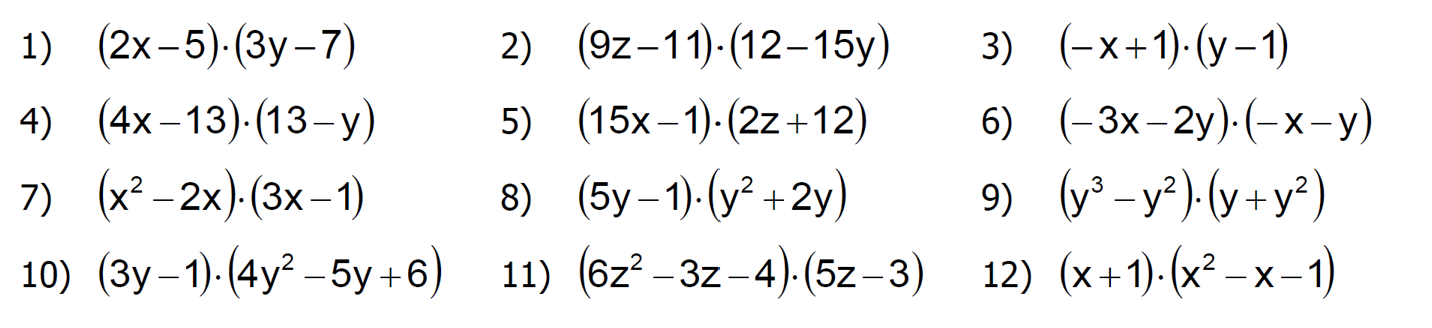
\includegraphics[scale=0.6]{molt-poli-1-25} }
		\solonly{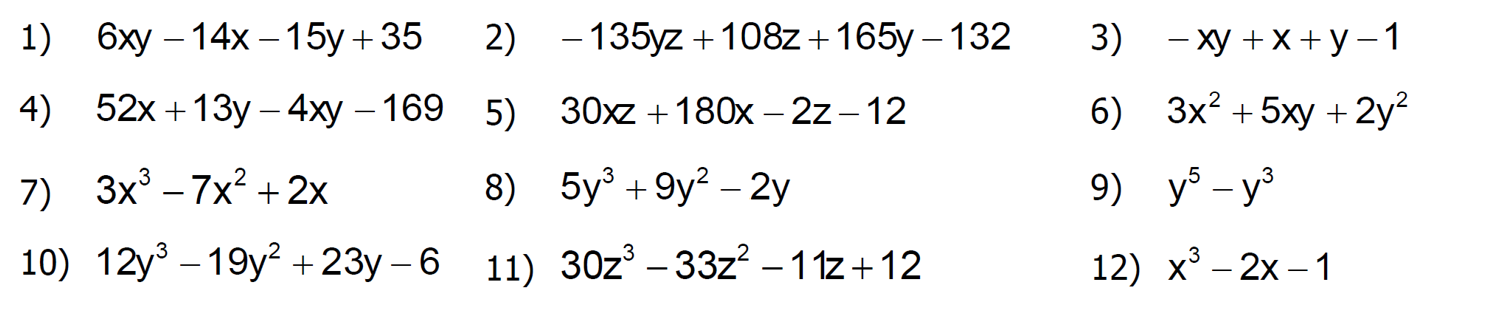
\includegraphics[scale=0.6]{molt-poli-1-25-sol} }

	\question
%TODO : convert in LaTeX
	\exonly{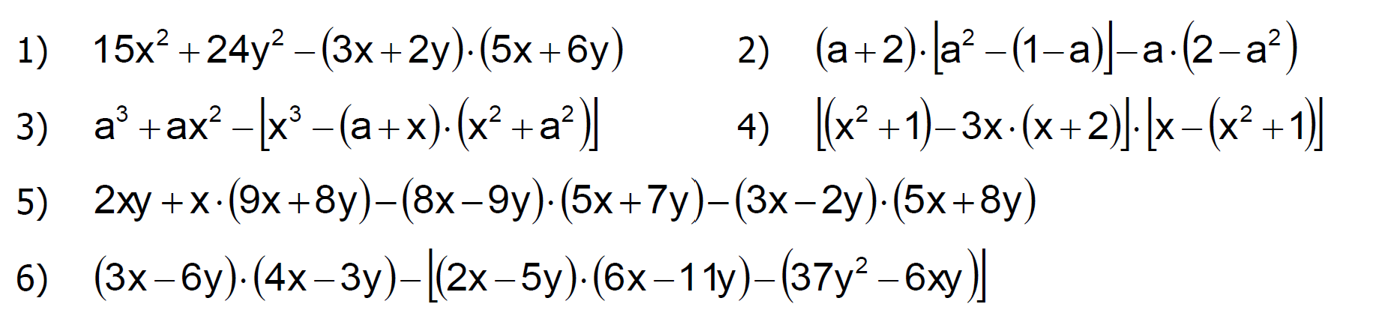
\includegraphics[scale=0.6]{molt-poli-1-26} }
	\solonly{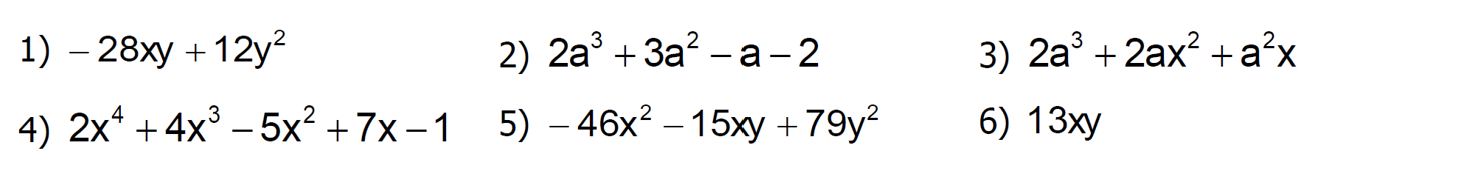
\includegraphics[scale=0.6]{molt-poli-1-26-sol} }

	\question
%TODO : convert in LaTeX
	\exonly{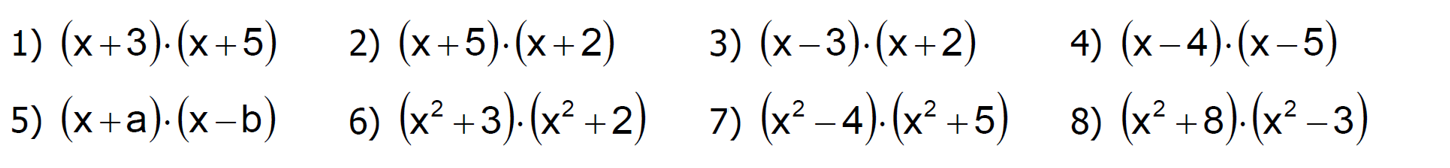
\includegraphics[scale=0.6]{molt-poli-1-27} }
	\solonly{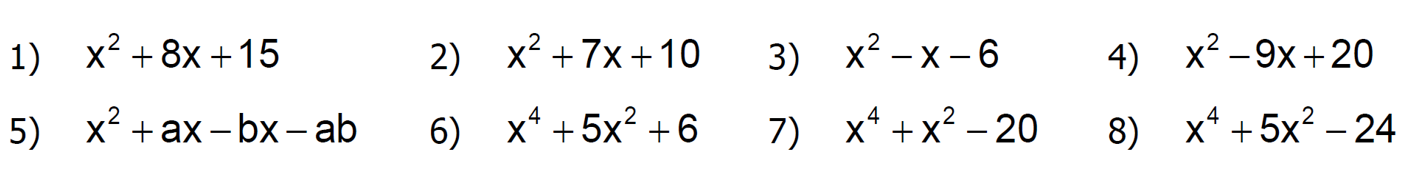
\includegraphics[scale=0.6]{molt-poli-1-27-sol} }
	
	\question

	\begin{parts}
		\part \exonly{$\dfrac{2}{5}x^2+ \dfrac{1}{4}x-2x+\dfrac{x^2}{10}=$}
		\solonly{$\dfrac{x^2}{2} - \dfrac{7}{4}x$}
		
		\part
		\exonly{$\dfrac{2}{3}\left( \dfrac{6x^2}{5}+12 \right) - \dfrac{4x}{3}\left(\dfrac{x^3}{2}-1\right)=$}
		\solonly{$-\dfrac{2x^4}{3}+\dfrac{4x^2}{5}+\dfrac{4x}{3}+8$}
		
		
		
		\part 
		\exonly{$3x- \dfrac{2}{3}x^2+ \dfrac{1}{12}x^2 + \dfrac{1}{2}x=$}
		\solonly{$-\dfrac{7x^2}{12} +\dfrac{7}{2}x$}
		
		\part
		\exonly{$\dfrac{5}{12}x + \dfrac{x}{6}-\dfrac{x}{3}+ \dfrac{1}{2}x=$}  \solonly{$\dfrac{3x}{4}$}
		
		\part
		
		\exonly{$\dfrac{1}{2}\left( 3x^3-5\right)-\dfrac{x}{3}\left(3x^3-6\right)+2x^2\left(\dfrac{x^2}{2}-\dfrac{5x}{4}-1\right)+ \dfrac{1}{2}=$ }
		\solonly{$-x^3-2x^2+2x-2 $}
	\end{parts}

	
	
\end{questions}

\newpage
\subsection{Fattorizzazione}

\begin{questions}
	
	\question 
	\exonly{Fattorizzare in $\Z[x]$ }
	
	\begin{minipage}{\linewidth}
		\begin{multicols}{2}
	\begin{parts}
		\part \exonly{$6 a+9$ } \solonly{$3(2 a+3)$ }
		\part \exonly{$15 t-10$ } \solonly{$5(3 t-2)$ }
		\part \exonly{$3 s^{2}+6 s$ } \solonly{$3 s(s+2)$ }
		\part \exonly{$12 x+16$ } \solonly{$4(3 x+4)$ }
		\part \exonly{$27 p+81$ } \solonly{$27(p+3)$ }
		\part \exonly{$18 a^{2} b^{2}-15 a^{2} b$ }  \solonly{$3 a^{2} b(6 b-5)$ }
		\part \exonly{$9 x-12$ } \solonly{$3(3 x-4)$ }
		\part \exonly{$x^{3}-x^{2}$ } \solonly{$x^{2}(x-1)$ }
		\part \exonly{$3 a^{3} b^{2}-6 a^{2} b$ } \solonly{$3 a^{2} b(a b-2)$ }
	\end{parts}
\end{multicols}
\end{minipage}

 \question \exonly{Fattorizzare  in $\Z[x]$ }
 
 	
 \begin{minipage}{\linewidth}
 	\begin{multicols}{2}
 \begin{parts}
 	\part \exonly{$x(y+3)+4(y+3)$ } \solonly{$(y+3)(x+4)$ }
  \part	\exonly{$x^{2}(2 t-1)+3(2 t-1)$ } \solonly{$(2 t-1)\left(x^{2}+3\right)$ }
  \part \exonly{$n(m-2)-(m-2)$ } \solonly{$(m-2)(n-1)$ }
  \part\exonly{$a^{2}(b+1)-a(b+1)$ } 
  \solonly{$a(b+1)(a-1)$ }
  \part \exonly{ $-2 p(q-1)+4(q-1)$  }
  \solonly{$(q-1)(-2 p+4)$ }
 \end{parts}
\end{multicols}
\end{minipage}


	\question \exonly{Fattorizzare in $\Z[x]$ }
	
%SRC : Favre es 3.3 pg 24 colonna 1
\begin{minipage}{\linewidth}
	\begin{multicols}{2}
		\begin{parts}
			\part
			\exonly{$a^{2}-9$ } \solonly{$(a-3)(a+3)$ }
			
		\part
		\exonly{$b^{2}-4 a^{2}$ } \solonly{$(b-2 a)(b+2 a)$ }
		\part
		\exonly{$x^{2}-6 x+9$ }	\solonly{ $(x-3)^{2}$ }
		
		\part
		\exonly{$1-x^{2}$ } \solonly{$(1-x)(1+x)$ }
		\part
		\exonly{$16 a^{2}-x^{2} y^{2}$ } \solonly{$(4 a-x y)(4 a+x y)$  }
		
		\part \exonly{$1+2 x^{2}+x^{4}$ } \solonly{$\left(x^{2}+1\right)^{2}$ }
		
		\part \exonly{$-144+b^{2} c^{2}$ } \solonly{$(b c-12)(b c+12)$ }
		\part \exonly{$a^{2}-9 b^{2} c^{4}$ } \solonly{$\left(a-3 b c^{2}\right)\left(a+3 b c^{2}\right)$ }
		
		\part
		\exonly{$9 x^{4}+16 y^{2}+24 x^{2} y$ }
		\solonly{ $\left(3 x^{2}+4 y\right)^{2}$ }
		
		\part
		\exonly{$x^4-81 $}
		\solonly{$(x-3)(x+3)(x^2+9)$ }
	\end{parts}
\end{multicols}
\end{minipage}


	\question \exonly{Fattorizzare in $\Z[x]$ }
	
	\begin{minipage}{\linewidth}
		\begin{multicols}{2}
	\begin{parts}
	
	\part 
	\exonly{$x^2 -6x-40$ }
	\solonly{$(x+4)(x-10)$ }
	
	
	\part 
	\exonly{$x^2 -13x+40$ }
	\solonly{$(x-5)(x-8)$ }
	
	\part
	\exonly{$x^2 +6x -55$ }
	\solonly{$(x-5)(x+11) $ }
	
	\part
	\exonly{$x^2 +7x -18$ }
	\solonly{$(x-2)(x+9)$ }

	
	
	\part
	\exonly{$x^2 -11x +28$ }
	 \solonly{$ (x-7)(x-4)$ }
	
	\part
	\exonly{$x^2 +7x +10$ }
	\solonly{$(x+5)(x+2)$ }

	
	\part
	\exonly{$x^2 -2x -48$ }
	\solonly{$(x+6)(x-8) $ }

	
	\part
	\exonly{$x^2 +2x-8$ }
	\solonly{$(x+4)(x-2) $ }

	
	\part
	\exonly{$x^2 +2x -3$ }
	\solonly{$(x+3)(x-1)$ }

	
	\part
	\exonly{$x^2 -12x +35$ }
	\solonly{$(x-5)(x-7)$ }

	
	\part
	\exonly{$x^2 +5x-36$ }
	\solonly{$(x-4)(x+9)$ }

	
	\part
	\exonly{$x^2 -7x+15$ }
	\solonly{Irriducibile in $\Z[x]$ }

	
	\part
	\exonly{$x^2 +23x +120$ }
	\solonly{$(x+15)(x+8)$ }

	
	\part
	\exonly{$x^2 -23x +132$ }
	\solonly{$(x-12)(x-11)$ }

	
	\part
	\exonly{$x^2+x-56$ }
	\solonly{$(x-7)(x+8)$ }

	
\end{parts}
\end{multicols}
\end{minipage}

% \exnewpage
% \solnewpage
\question
\exonly{Fattorizzare in $\Z[x]$  (valutazione formativa 1) }
 \solonly{ 
	I vari simboli ($\star$, \dots , $\Diamond$$\Diamond$$\Diamond$) permettono di raggruppare gli esercizi in funzione del metodo di fattorizzazione  da padroneggiare.
	
	$\star$: Messa in evidenza del MCD \\
	$\star\star$: Prodotti notevoli di grado 2 \\
%	$\star\star\star$: Prodotti notevoli di grado 3 \\
	$\Diamond$: Trinomio \\
%	$\Diamond\Diamond$: Raggruppamento\\
	$\Diamond\Diamond\Diamond$: Messa in evidenza e metodi vari
}

	\begin{minipage}{\linewidth}
	\begin{multicols}{2}
\begin{parts}
\part
\exonly{ $15x^{3} y^{4} +20x^{5} y^{4} -30x^{2} y^{3} =$}
\solonly{$\star$ $5x^{2} y^{3} \left(3xy+4x^{3} y-6\right)$}

\part  
\exonly{$64x^{2} +16x+1=$}
\solonly{$\star$$\star$ $\left(8x+1\right)^{2} $}

\part  
\exonly{$3x^{2} -18x-120=$}
\solonly{$\Diamond$ $3\left(x-10\right)\left(x+4\right)$}






\part  
\exonly{$49x^{2} -1=$}
\solonly{  $\star$$\star$ $\left(7x+1\right)\left(7x-1\right)$}

\part  
\exonly{$x^{2} -13x+40=$}
\solonly{  $\Diamond$ $\left(x-8\right)\left(x-5\right)$}




\part  
\exonly{$3x^{4} +60x^{3} +300x^{2} =$}
\solonly{  $\Diamond$$\Diamond$$\Diamond$ $3x^{2} \left(x+10\right)^{2} $}


			\part  
\exonly{$9x^{2} -25y^{2} =$}
\solonly{  $\star$$\star$ $\left(3x+5y\right)\left(3x-5y\right)$}


			\part  
\exonly{$27x^{3} -75x=$}
\solonly{  $\Diamond$$\Diamond$$\Diamond$ $3x\left(3x+5\right)\left(3x-5\right)$}



\part  
\exonly{$6x^{2} y^{3} +18x^{3} y^{4} -24x^{4} y^{3} =$}
\solonly{  $\star$ $6x^{2} y^{3} \left(1+3xy-4x^{2} \right)$}



\part
\exonly{$x^2-9x -20$ }
\solonly{ $\Diamond$ Irriducibile in $\Z[x]$ }




\part  
\exonly{$x^{2} +6x-55=$}
\solonly{  $\Diamond$ $\left(x+11\right)\left(x-5\right)$}



			\part  
\exonly{$121x^{2} -25=$}
\solonly{  $\star$$\star$ $\left(11x+5\right)\left(11x-5\right)$}


\part  
\exonly{$27x^{3} -12x=$}
\solonly{  $\Diamond$$\Diamond$$\Diamond$ $3x\left(3x+2\right)\left(3x-2\right)$}


		
		
\part  
\exonly{$x^{2} +7x-18=$}
\solonly{  $\Diamond$ $\left(x+9\right)\left(x-2\right)$}



\part  
\exonly{$12a^{4} b^{3} -6a^{2} b^{4} +24a^{3} b^{3} =$}
\solonly{  $\star$ $6a^{2} b^{3} \left(2a^{2} -b+4a\right)$}



	
	
	
\end{parts}

\end{multicols}
\end{minipage}




\question \exonly{Fattorizzare in $\Z[x]$ }

\begin{minipage}{\linewidth}
	\begin{multicols}{2}
		\begin{parts}
			\part
			\exonly{$2ax-6bx+ay-3by$ }
			\solonly{ $(a-3 b) (2 x+y) $}
			
			\part
			\exonly{$2ay^2-axy+6xy-3x^2$ }
			\solonly{$(2 y-x) (a y+3 x)$ }
			
			\part
			\exonly{$3x^3+3x^2-27x-27= $ }
			\solonly{$3 (x+1) (x-3) (x+3)$ }
			
			\part
			\exonly{$5x^3+10x^2-20x-40 $ }
			\solonly{$5 (x-2) (x+2)^2 $ }
			
			\part
			\exonly{	$x^4+2x^3-x-2$ }
			\solonly{$(x+2) (x-1) (x^2+x+1) $ }
			\part
			\exonly{$3 x^3 - 2 x^2 + 6 x - 4$ }
			\solonly{$(x^2+2)(3x-2) $ }
			
			
			\part
			\exonly{$4 x^3 + 8 x^2 - x - 2$ }
			\solonly{$(x+2)(2x-1)(2x+1)$ }
			
		\end{parts}
	\end{multicols}
\end{minipage}


% \solnewpage
\question
\exonly{Fattorizzare in $\Z[x]$  (valutazione formativa 2) }
\solonly{ 
	I vari simboli ($\star$, \dots , $\Diamond$$\Diamond$$\Diamond$) permettono di raggruppare gli esercizi in funzione del metodo di fattorizzazione  da padroneggiare.
	
	$\star$: Messa in evidenza del MCD \\
	$\star\star$: Prodotti notevoli di grado 2 \\
	$\star\star\star$: Prodotti notevoli di grado 3 \\
	$\Diamond$: Trinomio \\
	$\Diamond\Diamond$: Raggruppamento\\
	$\Diamond\Diamond\Diamond$: Messa in evidenza e metodi vari
}

\begin{minipage}{\linewidth}
	\begin{multicols}{2}
		\begin{parts}

			\part  
			\exonly{$27a^{3} +343=$}
			\solonly{$\star$$\star$$\star$ $\left(3a+7\right)\left(9a^{2} -21a+49\right)$}
			
			
			\part  
			\exonly{$36x^{2} -60x+25=$}
			\solonly{  $\star$$\star$ $\left(6x-5\right)^{2} $}
			
			
			\part  
			\exonly{$25x^{2} +40x+16=$}
			\solonly{  $\star$$\star$ $\left(5x+4\right)^{2} $}
			
			
			\part  
			\exonly{$8a^{2} -6ab+20ad-15bd=$}
			\solonly{  $\Diamond$$\Diamond$ $\left(4a-3b\right)\left(2a+5d\right)$}
			
			\part  
			\exonly{$125a^{3} -216=$ }
			\solonly{  $\star$$\star$$\star$ $\left(5a-6\right)\left(25a^{2} +30a+36\right)$} 		
			

			
			\part  
			\exonly{$216a^{3} -125=$ }
			\solonly{  $\star$$\star$$\star$ $\left(6a-5\right)\left(36a^{2} +30a+25\right)$} 
			
			

			
			
		\part  
			\exonly{$15x^{2} -10xy-9xz+6yz=$}
			\solonly{$\Diamond$$\Diamond$ $\left(5x-3z\right)\left(3x-2y\right)$}
			
			\part  
			\exonly{$8x^{3} -729=$}
			\solonly{  $\star$$\star$$\star$ $\left(2x-9\right)\left(4x^{2} +18x+81\right)$}
			
			\part  
			\exonly{$6a^{2} +15a-8ab-20b=$}
			\solonly{  $\Diamond$$\Diamond$ $\left(3a-4b\right)\left(2a+5\right)$}
			
			
			\part  
			\exonly{$15a^{3} b^{5} -10a^{2} b^{4} +20a^{3} b=$}
			\solonly{  $\star$ $5a^{2} b\left(3ab^{4} -2b^{3} +4a\right)$}
			
			

			
			
			\part  
			\exonly{$8a^{2} -6ab+20ad-15bd=$}
			\solonly{  $\Diamond$$\Diamond$ $\left(4a-3b\right)\left(2a+5d\right)$}
			
			
			\part  
			\exonly{$4x^{3} -32x^{2} +64x=$}
			\solonly{  $\Diamond$$\Diamond$$\Diamond$ $4x\left(x-4\right)^{2} $}
			
			
			\part  
			\exonly{$x^{2} -6x-40=$}
			\solonly{  $\Diamond$ $\left(x-10\right)\left(x+4\right)$}
			
			
			\part  
			\exonly{$27x^{3} +512=$ }
			\solonly{  $\star$$\star$$\star$ $\left(3x+8\right)\left(9x^{2} -24x+64\right)$} 
			
			
			\part  
			\exonly{$8x^{3} y^{3} +6x^{4} y^{5} -10x^{2} y^{4} =$}
			\solonly{  $\star$ $2x^{2} y^{3} \left(4x+3x^{2} y^{2} -5y\right)$}
			
			\part  
			\exonly{$8a^{2} +4ab-2ac-bc=$}
			\solonly{  $\Diamond$$\Diamond$ $\left(2a+b\right)\left(4a-c\right)$}
			
			
			

			
			\part  
			\exonly{$8x^{2} +10xy+4xz+5yz=$}
			\solonly{  $\Diamond$$\Diamond$ $\left(2x+z\right)\left(4x+5y\right)$}
			
			\part  
			\exonly{$x^{2} -11x+28=$}
			\solonly{  $\Diamond$ $\left(x-4\right)\left(x-7\right)$}
			
			\part  
			\exonly{$12x^{4} +60x^{3} +75x^{2} =$}
			\solonly{  $\Diamond$$\Diamond$$\Diamond$ $3x^{2} \left(2x+5\right)^{2} $}
			
			\part  
			\exonly{$27x^{3} -125=$}
			\solonly{$\star$$\star$$\star$$\left(3x-5\right)\left(9x^{2} +15x+25\right)$}	
			
		
		\part
		\exonly{$15 x^2 - x - 2=$}
		\solonly{$\Diamond$  $(5x-2)(3x+1)$}
		
			
			
		\end{parts}
		
	\end{multicols}
\end{minipage}
\end{questions}


% \exnewpage
\subsection{Applicazioni della fattorizzazione: frazioni algebriche}
\begin{questions}
\question
Semplificare le seguenti frazioni algebriche

% \exonly{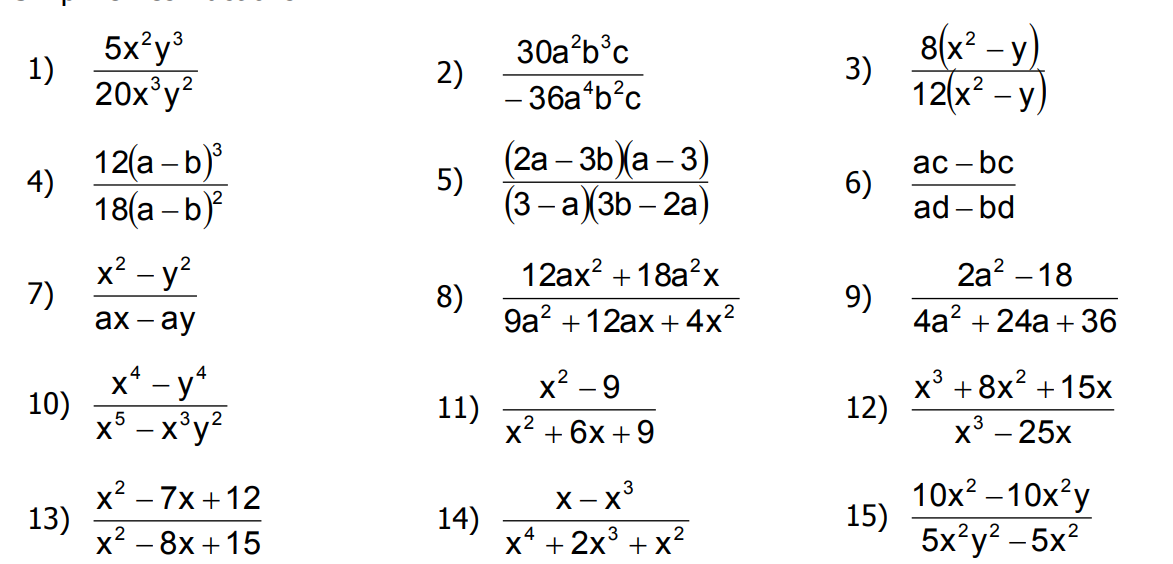
\includegraphics[scale=0.7]{frazioni-alg-4-1} }
% \solonly{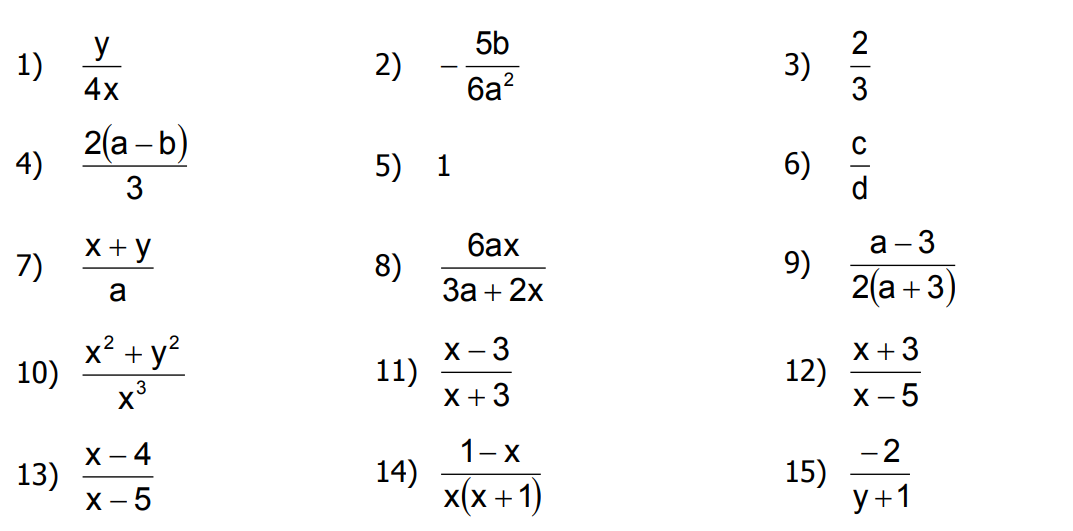
\includegraphics[scale=0.7]{frazioni-alg-4-1-sol} }
\begin{minipage}{\linewidth}
	\begin{multicols}{2}
		\begin{parts} %% Esercizio 4.1 EPAI
			\part
			\exonly{$\frac{5x^2y^3}{20x^3y^2}$}
			\solonly{$\frac{y}{4x}$} 

			\part
			\exonly{$\frac{30a^2b^3c}{-36a^4b^2c}$}
			\solonly{$-\frac{5b}{6a^2}$} 

			\part
			\exonly{$\frac{8(x^2-y)}{12(x^2-y)}$}
			\solonly{$\frac{2}{3}$} 

			\part
			\exonly{$\frac{12(a-b)^3}{18(a-b)^2}$}
			\solonly{$\frac{2(a-b)}{3}$} 

			\part
			\exonly{$\frac{(2a-3b)(a-3)}{(3-a)(3b-2a)}$}
			\solonly{$1$} 


			\part
			\exonly{$\frac{ac-bc}{ad-bd}$}
			\solonly{$\frac{c}{d}$} 

			\part
			\exonly{$\frac{x^2-y^2}{18(a-b)^2}$}
			\solonly{$\frac{x+y}{a}$} 

			\part
			\exonly{$\frac{12ax^2+18a^2x}{9a^2+12ax+4x^2}$}
			\solonly{$\frac{6ax}{3a+2x}$} 

			\part
			\exonly{$\frac{2a^2-18}{4a^2+24a+36}$}
			\solonly{$\frac{a-3}{2(a+3)}$} 

			\part
			\exonly{$\frac{x^4-y^4}{x^5-x^3y^2}$}
			\solonly{$\frac{x^2+y^2}{x^3}$} 

			\part
			\exonly{$\frac{x^2-9}{x^2+6x+9}$}
			\solonly{$\frac{x-3}{x+3}$} 

			\part
			\exonly{$\frac{x^3+8x^2+15x}{x^3-25x}$}
			\solonly{$\frac{x+3}{x-5}$} 

			\part
			\exonly{$\frac{x^2-7x+12}{x^2-8x+15}$}
			\solonly{$\frac{x-4}{x-5}$} 

			\part
			\exonly{$\frac{x-x^3}{x^4+2x^3+x^2}$}
			\solonly{$\frac{1-x}{x(x+1)}$} 

			\part
			\exonly{$\frac{10x^2-10x^2y}{5x^2y^2-5x^2}$}
			\solonly{$\frac{-2}{y+1}$} 

			
			
		\end{parts}
	\end{multicols}
\end{minipage}	


\question
Effettuare e semplificare

% \exonly{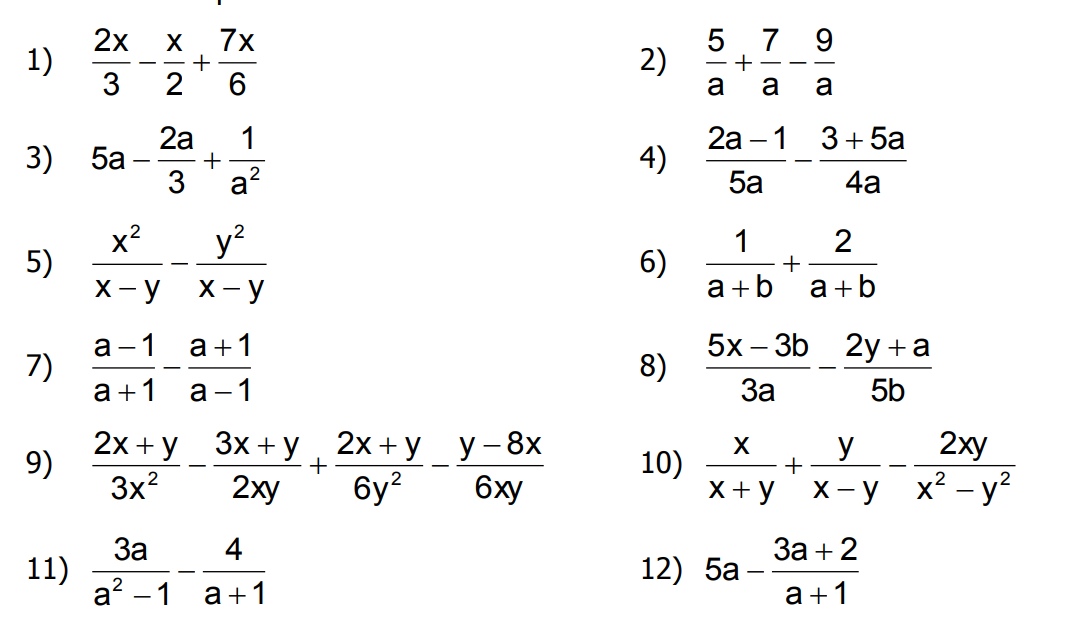
\includegraphics[scale=0.7]{frazioni-alg-4-2} }
% \solonly{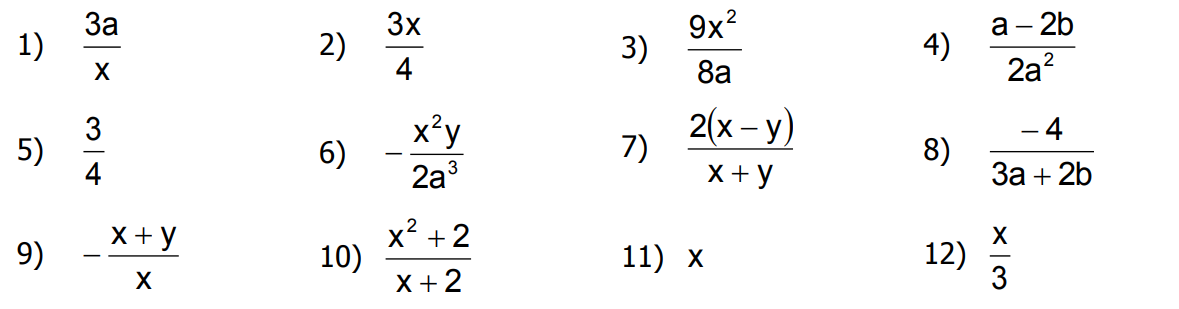
\includegraphics[scale=0.7]{frazioni-alg-4-2-sol} }


\begin{minipage}{\linewidth}
	\begin{multicols}{2}
		\begin{parts} %% Esercizio 4.4 EPAI
			\part
			\exonly{$\frac{2x}{3}-\frac{x}{2}+\frac{7x}{6}$}
			\solonly{$\frac{4x}{3}$} 

			\part
			\exonly{$\frac{5}{a}+\frac{7}{a}-\frac{9}{a}$}
			\solonly{$\frac{3}{a}$} 

			\part
			\exonly{$5a-\frac{2a}{3}+\frac{1}{a^2}$}
			\solonly{$\frac{13a^3+3}{3a^2}$} 

			\part
			\exonly{$\frac{2 a-1}{5 a}-\frac{3+5 a}{4 a}$}
			\solonly{$-\frac{17 a+19}{20 a}$} 

			\part
			\exonly{$\frac{x^2}{x-y}-\frac{y^2}{x-y}$}
			\solonly{$x+y$} 

			\part
			\exonly{$\frac{1}{a+b}+\frac{2}{a+b}$}
			\solonly{$\frac{3}{a+b}$} 

			\part
			\exonly{$\frac{a-1}{a+1}-\frac{a+1}{a-1}$}
			\solonly{$\frac{-4a}{(a+1)(a-2)}$} 

			\part
			\exonly{$\frac{5 x-3 b}{3 a}-\frac{2 y+a}{5 b}$}
			\solonly{$\frac{25bx-15b^2-6ay-3a^2}{15ab}$} 

			\part
			\exonly{$\frac{2 x+y}{3 x^2}-\frac{3 x+y}{2 x y}+\frac{2 x+y}{6 y^2}-\frac{y-8 x}{6 x y}$}
			\solonly{$\frac{x^3+y^3}{3x^2y^2}$} 

			\part
			\exonly{$\frac{x}{x+y}+\frac{y}{x-y}-\frac{2 x y}{x^2-y^2}$}
			\solonly{$\frac{x-y}{x+y}$} 

			\part
			\exonly{$\frac{3 a}{a^2-1}-\frac{4}{a+1}$}
			\solonly{$\frac{-a+4}{(a+1)(a-1)}$} 

			\part
			\exonly{$5 a-\frac{3 a+2}{a+1}$}
			\solonly{$\frac{5a^2+2a-2}{a+1}$} 
			
		\end{parts}
	\end{multicols}
\end{minipage}		

	



	
\end{questions}


\end{document}